\documentclass[11pt]{article}
\usepackage[margin=2.5cm]{geometry}
\usepackage{amsmath,amssymb,amsthm}
\usepackage{booktabs}
\usepackage{graphicx}
\usepackage{xurl}
\usepackage[hidelinks]{hyperref}

\newcommand{\Z}{\mathbb{Z}}
\newtheorem{theorem}{Theorem}
\newtheorem{proposition}[theorem]{Proposition}
\newtheorem{lemma}[theorem]{Lemma}
\newtheorem{corollary}[theorem]{Corollary}
\theoremstyle{remark}
\newtheorem{remark}[theorem]{Remark}

\title{On two open points in Part IV of Ramanujan's Lost Notebook:\\ the domain of Entry 12.2.3 and a summation reading of Entry 19.2.2}
\author{Otakhon U. Kenjaev\\ \small Independent researcher, Khorezm, Uzbekistan\\
\small ORCID \href{https://orcid.org/0009-0009-3566-9285}{0009-0009-3566-9285}}
\date{September 2026}

\begin{document}
\maketitle

\begin{abstract}
We discuss two places in Andrews and Berndt, \emph{Ramanujan's Lost Notebook, Part IV}, where a question is left open.
(1) For Entry 12.2.3, $L(s,\chi)L(s-r,\chi)=\sum\chi(n)\sigma_r(n)n^{-s}$ with $\chi$ the non-principal character modulo $4$,
the authors expect the identity to hold for $\operatorname{Re}s>\sup\{0,\operatorname{Re}r\}$. We show that this fails for $r=0$:
the abscissa of convergence of $\sum\chi(n)d(n)n^{-s}$ lies in $[\tfrac14,\tfrac13]$, so the series diverges for
$0<\operatorname{Re}s<\tfrac14$ although both series on the left converge there. The proof combines Kronecker's lemma with a
mean-square theorem of Cao, Tanigawa and Zhai and an upper bound of de Roton. (2) For Entry 19.2.2, which the authors call false
because it contains divergent series, we show that for $s<-2$ and quadratic irrational $\alpha/2\pi$ the series
$\sum\sigma_s(n)\sin(n\alpha)$ is Abel summable, with value $\frac12\sum_d d^s\cot(d\alpha/2)$, but that the identity still fails
with this reading; numerically the value has poles at the rational points $\alpha/2\pi=p/q$, which suggests why an identification
with the smooth double integral in (19.4.2) was not found. A verification script accompanies the note.
\end{abstract}

\noindent\textit{2020 Mathematics Subject Classification:} 11M41, 11N37, 40G10, 01A60.\\
\textit{Keywords:} Ramanujan's lost notebook, Dirichlet series, abscissa of convergence, mean square, Abel summation.

\section{Introduction}
Chapter 12 of \cite{AB4} records a manuscript of Ramanujan on infinite series. With $\chi$ the non-principal character modulo $4$ and
$\sigma_r(n)=\sum_{d\mid n}d^r$, Entry 12.2.3 (p.~318 of \cite{LN}) states that for $\operatorname{Re}s>1$, $\operatorname{Re}(s-r)>1$,
\begin{equation}\label{eq:1223}
\sum_{m\ge1}\frac{\chi(m)}{m^s}\sum_{n\ge1}\frac{\chi(n)}{n^{s-r}}=\sum_{n\ge1}\frac{\chi(n)\sigma_r(n)}{n^s}.
\end{equation}
After the (easy) proof the authors write: ``We expect that the domain of validity can be extended to
$\operatorname{Re}s>\sup\{0,\operatorname{Re}r\}$, but we are unable to prove this'' \cite[p.~270]{AB4}. This is the region where
both series on the left converge. In Section~\ref{sec:1223} we show that the expectation fails already for $r=0$.

Chapter 19 of \cite{AB4} begins with two formulas from page 336 of \cite{LN} that are ``clearly wrong'' because they contain
divergent series. The second, Entry 19.2.2, asserts that for $\alpha,\beta>0$ with $\alpha\beta=4\pi^2$,
\begin{multline}\label{eq:1922}
\alpha^{(s+1)/2}\Bigl\{\tfrac1\alpha\zeta(1-s)+\tfrac12\zeta(-s)\tan\tfrac{\pi s}2+\sum_{n\ge1}\sigma_s(n)\sin(n\alpha)\Bigr\}\\
=\beta^{(s+1)/2}\Bigl\{\tfrac1\beta\zeta(1-s)+\tfrac12\zeta(-s)\tan\tfrac{\pi s}2+\sum_{n\ge1}\sigma_s(n)\sin(n\beta)\Bigr\}.
\end{multline}
Andrews and Berndt compare it with Ramanujan's correct formula (19.4.1), which has a double integral in place of the series, and
write that they ``are unable to make any identification of the double integrals in (19.4.2) with the divergent sums in (19.2.2)''
\cite[p.~380]{AB4}. In Section~\ref{sec:1922} we test the most natural reading of the divergent series, by Abel summation.

We do not claim new methods; both points are applications of standard tools. We found no discussion of either point in the
literature citing \cite{AB4} (zbMATH Open, OpenAlex, September 2026).

\section{Entry 12.2.3 with \texorpdfstring{$r=0$}{r=0}}\label{sec:1223}
Let $A(x)=\sum_{n\le x}\chi(n)d(n)$ and let $\sigma_c$ be the abscissa of convergence of $F(s)=\sum_{n\ge1}\chi(n)d(n)n^{-s}$.
For $\operatorname{Re}s>1$, $F(s)=L(s,\chi)^2$.

\begin{theorem}\label{thm:main}
$\tfrac14\le\sigma_c\le\tfrac13$. Consequently $F(s)$ diverges for every $s$ with $\operatorname{Re}s<\tfrac14$, and \eqref{eq:1223}
with $r=0$ holds for $\operatorname{Re}s>\tfrac13$ but not for $0<\operatorname{Re}s<\tfrac14$, although $\sum\chi(m)m^{-s}$ converges
for $\operatorname{Re}s>0$.
\end{theorem}

The lower bound is a consequence of classical $\Omega$-results for Dirichlet series with a functional equation of this
type (Landau \cite{La}; Chandrasekharan and Narasimhan \cite{CN}); we derive it from a recent mean-square theorem whose hypotheses
can be checked directly. We use the class $S^\theta_{\rm real}$ of Cao, Tanigawa and Zhai \cite{CTZ}: Dirichlet series $L(s)=\sum a(n)n^{-s}$ with real
coefficients such that $(s-1)^mL(s)$ is entire of finite order for some $m\ge0$; $\Lambda(s)=L(s)Q^s\prod_{j}\Gamma(\alpha_js+\beta_j)$
satisfies $\Lambda(s)=\omega\Lambda(1-\bar s)$ with $Q>0$, $|\omega|=1$, $\alpha_j>0$, $\operatorname{Re}\beta_j\ge0$, $\sum\beta_j$ real;
and $|a(n)|\ll n^{\theta+\varepsilon}$, $\sum_{n\le y}|a(n)|^2\ll y^{1+\varepsilon}$. The degree is $d=2\sum\alpha_j$. The error term is
$E(y)=A^*(y)-Q(y)$, where $A^*(y)=\sum_{n\le y}{}'a(n)$ (last term halved when $y$ is an integer) and $Q(y)$ is the sum of the residues
of $L(s)y^s/s$.

\begin{lemma}\label{lem:class}
$L(s,\chi)^2\in S^0_{\rm real}$, of degree $2$, and $Q(y)=\tfrac14$.
\end{lemma}

\begin{proof}
$L(s,\chi)$ is entire of finite order, and since $\chi$ is odd and primitive of conductor $4$ with root number $1$,
$\xi(s)=(4/\pi)^{s/2}\Gamma(\tfrac{s+1}2)L(s,\chi)$ satisfies $\xi(s)=\xi(1-s)$. Hence $\Lambda(s)=(4/\pi)^s\Gamma(\tfrac{s+1}2)^2L(s,\chi)^2$
satisfies $\Lambda(s)=\Lambda(1-s)$, with $\alpha_1=\alpha_2=\beta_1=\beta_2=\tfrac12$, $Q=4/\pi$, $\omega=1$, $d=2$. The coefficients
$\chi(n)d(n)$ are real, $|\chi(n)d(n)|\le d(n)\ll n^\varepsilon$ and $\sum_{n\le y}d(n)^2\ll y\log^3y$. The only pole of $L(s,\chi)^2y^s/s$
is at $s=0$, with residue $L(0,\chi)^2=\tfrac14$.
\end{proof}

\begin{proof}[Proof of Theorem~\ref{thm:main}]
By \cite[Corollary~1]{CTZ} (degree $2$, $\theta=0\le\tfrac14$) and Lemma~\ref{lem:class},
\begin{equation}\label{eq:ms}
\int_1^TE(y)^2\,dy=C_2T^{3/2}+O(T^{1+\varepsilon}),\qquad C_2>0.
\end{equation}
Suppose $\sigma_c<\tfrac14$ and choose a real $s_0$ with $\max\{\sigma_c,0\}<s_0<\tfrac14$. Then $\sum\chi(n)d(n)n^{-s_0}$ converges,
so $A(x)=o(x^{s_0})$ by Kronecker's lemma (partial summation), hence $E(y)=o(y^{s_0})$ and $\int_1^TE^2=o(T^{1+2s_0})=o(T^{3/2})$,
contradicting \eqref{eq:ms}. Thus $\sigma_c\ge\tfrac14$; a Dirichlet series that converges at $s_1$ converges for
$\operatorname{Re}s>\operatorname{Re}s_1$, so $F$ diverges whenever $\operatorname{Re}s<\tfrac14$. For the upper bound, $L(s,\chi)^2$
lies in the extended Selberg class, so de Roton's estimate \cite{dR} (as stated in \cite[\S1.1]{CTZ}) gives $E(y)\ll y^{(d-1)/(d+1)+\varepsilon}=y^{1/3+\varepsilon}$;
partial summation then gives convergence of $F(s)$ for $\operatorname{Re}s>\tfrac13$, and $F(s)=L(s,\chi)^2$ there by analytic
continuation.
\end{proof}

\begin{remark}\label{rem:r}
For real $r$ the same heuristic, applied to $L(s+\tfrac r2,\chi)L(s-\tfrac r2,\chi)=\sum\chi(n)\sigma_r(n)n^{-r/2}\,n^{-s}$, predicts
divergence of the right side of \eqref{eq:1223} for $\sup\{0,r\}<s<\tfrac14+\tfrac r2$, an interval that is non-empty exactly when
$|r|<\tfrac12$. Numerically, with $A_r(x)=\sum_{n\le x}\chi(n)\sigma_r(n)$, the mean of $A_r(x)^2/x^{1/2+r}$ over $[X/2,X]$ is of order $1$ for
$r=\pm\tfrac14$ and $X=10^5,10^6$ (check A6 of the script). We do not claim this case: the coefficients $\chi(n)\sigma_r(n)n^{-r/2}$ do not satisfy
$\sum_{n\le y}|a(n)|^2\ll y^{1+\varepsilon}$ when $r\ne0$, so \cite[Corollary~1]{CTZ} does not apply as stated.
\end{remark}

Table~\ref{tab:ms} illustrates \eqref{eq:ms}; $A(x)$ is computed exactly by the hyperbola method
\[
A(x)=2\sum_{a\le\sqrt x}\chi(a)S(x/a)-S(\sqrt x)^2,\qquad S(m)=\sum_{b\le m}\chi(b).
\]
The partial sums of $\sum\chi(n)d(n)n^{-1/5}$ oscillate
with range $8.970$, $10.795$, $14.929$ on $[10^k,10^{k+1}]$, $k=3,4,5$ (Figure~\ref{fig:ln4}, left).

\begin{figure}[ht]
\centering
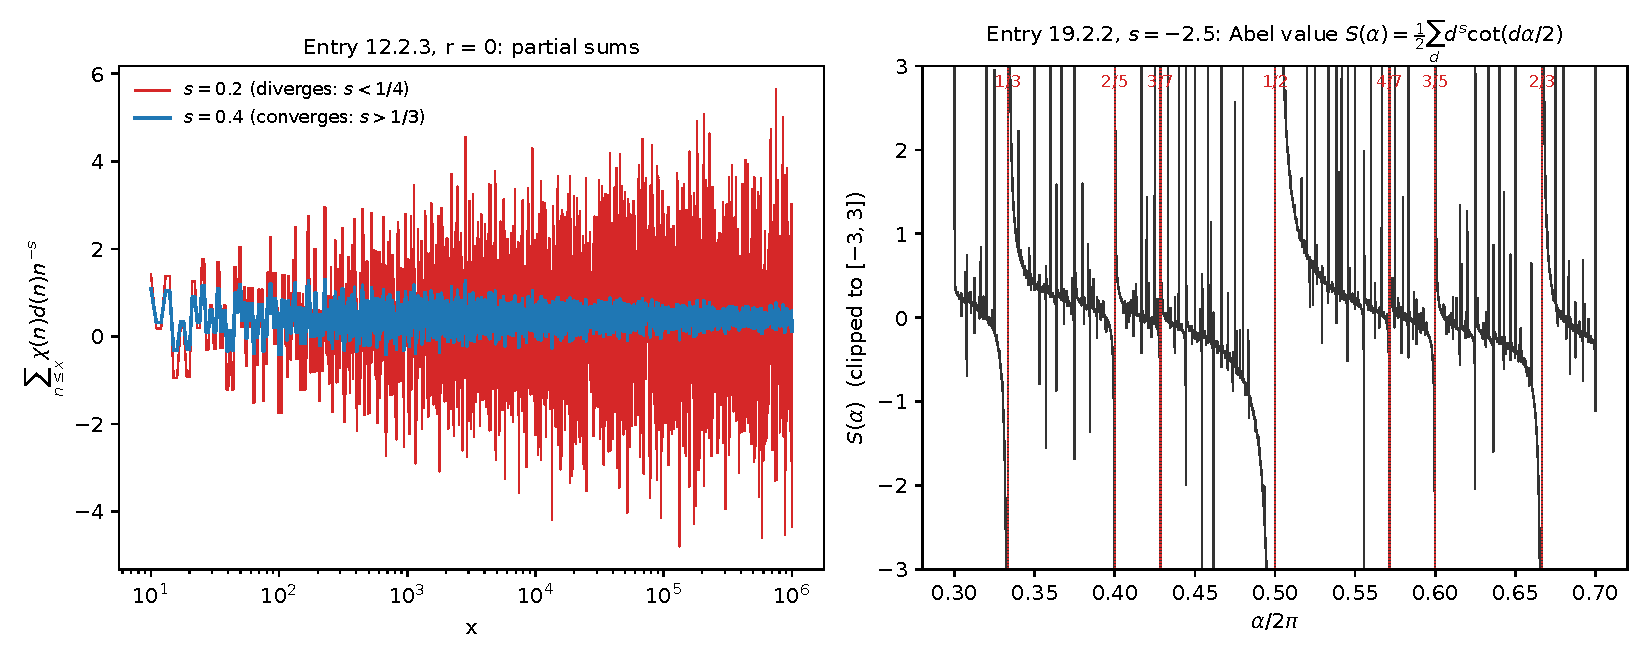
\includegraphics[width=\textwidth]{ln4_remarks.pdf}
\caption{Left: partial sums of $\sum\chi(n)d(n)n^{-s}$ for $s=0.2$ (divergent, Theorem~\ref{thm:main}) and $s=0.4$ (convergent).
Right: the Abel value $S(\alpha)$ of Section~\ref{sec:1922} for $s=-2.5$, with poles at rational $\alpha/2\pi$.}\label{fig:ln4}
\end{figure}

\begin{table}[ht]
\centering
\begin{tabular}{lcccc}
\toprule
$X$ & $10^6$ & $10^8$ & $10^{10}$ & $10^{12}$\\
\midrule
mean of $A(x)^2/\sqrt x$ over 600 random $x\in[X/2,X]$ & $0.7322$ & $0.7815$ & $0.7571$ & $0.8151$\\
\bottomrule
\end{tabular}
\caption{The mean square of $A(x)$ is of order $x^{1/2}$, as in \eqref{eq:ms}.}\label{tab:ms}
\end{table}

\section{Entry 19.2.2 read by Abel summation}\label{sec:1922}
Put $\xi=\alpha/2\pi$ and $S(\alpha)=\tfrac12\sum_{d\ge1}d^s\cot(d\alpha/2)$.

\begin{proposition}\label{prop:abel}
Let $s<-2$ and let $\xi$ be irrational with $\|d\xi\|\ge c/d$ for all $d\ge1$ and some $c>0$ (for example, $\xi$ a quadratic irrational).
Then $S(\alpha)$ converges absolutely and $\sum_{n\ge1}\sigma_s(n)\sin(n\alpha)$ is Abel summable to $S(\alpha)$.
\end{proposition}

\begin{proof}
For $0<t<1$ and $\beta\notin2\pi\Z$ put $f_t(\beta)=\sum_{m\ge1}t^m\sin(m\beta)=t\sin\beta/(1-2t\cos\beta+t^2)$. Since
$1-2t\cos\beta+t^2\ge4t\sin^2(\beta/2)$, we have $|f_t(\beta)|\le1/(2|\sin(\beta/2)|)$, and $f_t(\beta)\to\tfrac12\cot(\beta/2)$ as $t\to1^-$.
With $\beta=d\alpha$, $|\sin(\pi d\xi)|\ge2\|d\xi\|\ge2c/d$, so $|d^sf_t(d\alpha)|\le d^{s+1}/(4c)$, which is summable for $s<-2$. As
$\sigma_s$ is bounded, $\sum_n\sigma_s(n)\sin(n\alpha)t^n=\sum_dd^sf_{t^d}(d\alpha)$ for $0<t<1$, and dominated convergence gives the limit
$S(\alpha)$ as $t\to1^-$.
\end{proof}

Since Ces\`aro $(C,1)$ summability implies Abel summability with the same value \cite{Hardy}, the $(C,1)$ reading of \eqref{eq:1922},
where it exists, gives the same numbers. Let $\mathcal L(\alpha)$ denote the left side of \eqref{eq:1922} with the series replaced by
$S(\alpha)$.

\begin{corollary}\label{cor:fail}
Entry 19.2.2 is false also in the Abel reading. For $s=-2.5$ and $\alpha=2\pi\sqrt2$, $\beta=4\pi^2/\alpha$,
$\mathcal L(\alpha)-\mathcal L(\beta)=0.1408\ldots$; similarly $0.0658$ and $-0.0464$ for $\xi=\tfrac{1+\sqrt5}2$ and $\sqrt3$, and
$0.0422$, $0.0305$, $0.0211$ for $s=-4.5$.
\end{corollary}

\begin{proof}
$\xi$ and $1/\xi$ are quadratic irrationals, so Proposition~\ref{prop:abel} applies to both $\alpha$ and $\beta$. If the partial quotients of $\xi$ are
bounded by $M$, then $\|d\xi\|>1/((M+2)d)$ for all $d\ge1$ \cite{Kh}; here $M\le2$, so $c=\tfrac14$ is admissible for $\xi$ and $1/\xi$.
Truncating $S$ at $d\le D=4\cdot10^6$, the tail is at most $\sum_{d>D}d^{s+1}/(4c)\le D^{s+2}/(-s-2)$. The total truncation error is
below $10^{-3}$ for $s=-2.5$ and below $10^{-17}$ for $s=-4.5$, far smaller than the differences stated.
\end{proof}

\begin{remark}\label{rem:poles}
The terms with $q\mid d$ suggest that $S$ has a pole at each $\alpha_0=2\pi p/q$ with residue $q^{s-1}\zeta(1-s)$. Numerically,
for $s=-2.5$ and $\alpha=\alpha_0+10^{-6}$, $(\alpha-\alpha_0)S(\alpha)$ agrees with $q^{s-1}\zeta(1-s)$ (see also Figure~\ref{fig:ln4}, right) to relative accuracy
$1.4\cdot10^{-10}$, $1.0\cdot10^{-5}$, $2.0\cdot10^{-5}$, $3.3\cdot10^{-5}$ for $p/q=\tfrac12,\tfrac13,\tfrac25,\tfrac37$. The double
integral in (19.4.1), by contrast, is a smooth function of $\alpha>0$ for $s>-1$, and its analytic continuation to $-3<s<-1$
(computed numerically) shows no such singularities. So the divergent series in \eqref{eq:1922} cannot be matched
pointwise with the double integrals under this reading, which may explain why no identification was found.
\end{remark}

\medskip\noindent\textbf{Data availability.} The script \texttt{verify\_ln4\_remarks.py} (10 checks, requiring NumPy and mpmath)
reproduces every number in this note, including Table~\ref{tab:ms}; an offline calculator for $A(x)$ and for the two sides of
\eqref{eq:1922}, and the code for Figure~\ref{fig:ln4} are available at
\url{https://github.com/selloriybrendi/ramanujan-lost-notebook-iv-remarks}; the calculator runs at
\url{https://selloriybrendi.github.io/ramanujan-lost-notebook-iv-remarks/}.

\section*{Use of generative AI}
Claude Opus 5.5 (Anthropic, model identifier \texttt{claude-opus-5-5}), accessed through Claude Code in September 2026, was used to
locate the open questions in \cite{AB4}, to find the mean-square theorem in \cite{CTZ} and check its hypotheses, to carry out the
numerical computations reported here (with NumPy and mpmath) under the author's direction, and to help prepare the text. It was used
to verify every stated number independently. The author directed the work, checked all results and takes full responsibility for
the content.

\begin{thebibliography}{9}
\bibitem{LN} S. Ramanujan, \emph{The Lost Notebook and Other Unpublished Papers}, Narosa, New Delhi, 1988.
\bibitem{AB4} G. E. Andrews and B. C. Berndt, \emph{Ramanujan's Lost Notebook, Part IV}, Springer, New York, 2013, Chapters 12 and 19.
\bibitem{CTZ} X. Cao, Y. Tanigawa and W. Zhai, Tong-type identity and the mean square of the error term for an extended Selberg class,
\emph{Sci. China Math.} 59 (2016), 2103--2144; \href{https://arxiv.org/abs/1501.04269}{arXiv:1501.04269}.
\bibitem{dR} A. de Roton, On the mean square of the error term for an extended Selberg class, \emph{Acta Arith.} 126 (2007), 27--55.
\bibitem{Hardy} G. H. Hardy, \emph{Divergent Series}, Clarendon Press, Oxford, 1949.
\bibitem{La} E. Landau, \"Uber die Anzahl der Gitterpunkte in gewissen Bereichen, \emph{Nachr. Ges. Wiss. G\"ottingen} (1912),
687--771.
\bibitem{CN} K. Chandrasekharan and R. Narasimhan, On the mean value of the error term for a class of arithmetical functions,
\emph{Acta Math.} 112 (1964), 41--67.
\bibitem{Kh} A. Ya. Khinchin, \emph{Continued Fractions}, University of Chicago Press, Chicago, 1964.
\end{thebibliography}
\end{document}
